\chapter{Building a groundwater model from Raven inputs}\label{uch:build}
In this mode Raven builds the MODFLOW~6 model for you. You describe the aquifer in the \cmd{.rvp} file, give maps in
the \cmd{.rvg} file, and Raven makes the grid, the layers and every MODFLOW file. This chapter says what to write and
which choices matter. Reference, Chapter~\ref{R-ch:c3}, gives every rule of the model builder. Workshop~2 builds such a
model for a small Raven model, Tutorial Creek.

\section{Which HRUs are coupled}
An HRU is \emph{coupled} when its \cmd{AQUIFER\_PROFILE} in the \cmd{.rvh} file names a profile defined in the \cmd{.rvp}
file. HRUs with \cmd{[NONE]} (or an empty entry) keep Raven's usual behaviour. Disabled HRUs are never coupled (Raven
prints a warning).

Raven checks two rules about the \cmd{GROUNDWATER} store at start-up:
\begin{itemize}
\item No Raven process may take water \emph{out of} \cmd{GROUNDWATER} in a coupled HRU, because MODFLOW owns that water.
Raven stops with an error naming the process.
\item A process that sends water \emph{into} \cmd{GROUNDWATER} in an uncoupled HRU makes that water leave the model.
Raven warns, so that you can restrict the process with \cmd{:-->Conditional}.
\end{itemize}
\begin{inpractice}
Define an HRU group of the coupled HRUs, send percolation to \cmd{GROUNDWATER} only in that group, and keep the old
process for the other HRUs. Step~3 of Chapter~\ref{uch:quick} shows the two lines.
\end{inpractice}

\section{Describing the aquifer}\label{sec:uprofiles}
Three blocks in the \cmd{.rvp} file describe the ground below the HRUs.

\paragraph{Aquifer classes} are materials. Each has a horizontal conductivity \cmd{K\_HORIZ} (required) and, if you want,
\cmd{K\_VERT} (default $K_h/10$), \cmd{SPEC\_STORAGE} (default $10^{-5}$ 1/m) and \cmd{SPEC\_YIELD} (default 0.1).
\cmd{POROSITY}, \cmd{CLAPP\_B} and \cmd{AIR\_ENTRY\_PRESSURE} are used only by the unsaturated columns of the soil zone
(Section~\ref{sec:usoilzone}). Classes must be defined before the profiles that use them.

\paragraph{Aquifer profiles} are layer stacks. Each row gives the profile's name, its number of layers, then for each
layer, from the top down, a class, a thickness in metres (or \cmd{TO\_BEDROCK}) and a layer type: \cmd{AQUIFER} (or
\cmd{UNCONFINED\_AQUIFER}), \cmd{CONFINED\_AQUIFER}, \cmd{AQUITARD} or \cmd{AQUICLUDE} (not as top layer).

\paragraph{Aquifer profile parameters} set, per profile, how the model starts and how it exchanges water: the initial
depth to water (\cmd{INITIAL\_HEAD\_DEPTH}, 5~m), the depth of bedrock where there is no bedrock map
(\cmd{DEFAULT\_BEDROCK\_DEPTH}, 50~m), the seepage leakance (\cmd{SEEPAGE\_LEAKANCE}, 1/d), the riverbed
(\cmd{RIVERBED\_K}, \cmd{RIVERBED\_THICKNESS}), evaporation from the water table (\cmd{EXTINCTION\_DEPTH}) and a recharge
delay (\cmd{RECHARGE\_DELAY}). Reference, Sections~\ref{R-app:class} and~\ref{R-app:profile}, list every parameter
with its default, its checked range and typical values.

\paragraph{How the layers are stacked.} For each active column Raven takes the land surface from the DEM (or, without a
DEM, the HRU elevations) and bedrock from the bedrock map (or \cmd{DEFAULT\_BEDROCK\_DEPTH} below the land). The model top
is the land surface, lowered by \cmd{SOIL\_ZONE\_DEPTH} when you give one. The layers of the column's profile (the
profile of its dominant HRU) are then laid down from the top, each with its thickness, and never below bedrock. A layer
marked \cmd{TO\_BEDROCK} reaches bedrock. Where bedrock cuts a layer off completely, that layer becomes a very thin
\emph{pass-through} cell, so water passes straight from the layer above to the layer below. A column whose bedrock lies
less than 0.5~m below its top is inactive.

\begin{example}[: one column]
Land surface 600~m, bedrock 555~m, profile \cmd{VALLEY\_ALLUVIUM} = gravel 15~m, clay till 5~m, sand \cmd{TO\_BEDROCK}.
The gravel runs from 600 to 585~m, the till from 585 to 580~m, the sand from 580 to 555~m. If bedrock were at 582~m,
the till would end at 582~m (3~m thick) and the sand would have no thickness left: it becomes a pass-through cell.
\end{example}

\begin{watch}
By default (\cmd{:LayerConnection INDEX}) MODFLOW connects layer~$\ell$ of one column sideways only to layer~$\ell$ of its
neighbours. Where two profiles meet, list their layers in the same geological order, otherwise, for example, a gravel layer
may connect to a clay layer. Or use \cmd{:LayerConnection ELEVATION}, which connects the cells whose elevations overlap
(Reference, Section~\ref{R-sec:layerconn}).
\end{watch}

\section{Maps}\label{sec:umaps}
\subsection{HRU polygons}
The HRU polygons are required (\cmd{:HRUGeometry file ID\_field}). Raven's HRUs usually come from a GIS overlay (for
example BasinMaker): subbasins intersected with land-use, soil and terrain classes. Export that polygon layer as a GeoJSON
file, keeping the HRU ID used in the \cmd{.rvh}:
\par\noindent\begin{minipage}{\linewidth}
\begin{lstlisting}
ogr2ogr -f GeoJSON -t_srs EPSG:4326 my_hrus.geojson my_hrus.shp
\end{lstlisting}
\end{minipage}\par\smallskip
(or, in QGIS, \emph{Export $\rightarrow$ Save Features As}, format GeoJSON, CRS EPSG:4326). A layer in a projection may
also be exported as it is (\cmd{ogr2ogr -f GeoJSON my\_hrus.geojson my\_hrus.shp}) and its projection given by
\cmd{:InputCRS} in the \cmd{.rvg} file (Section~\ref{sec:uinputcrs}).

Check that every HRU with an \cmd{AQUIFER\_PROFILE} appears in the file. Only those HRUs need polygons; others may be
present and are ignored. \cmd{GWModelSummary.txt} lists, per HRU, its polygon area, its area in the \cmd{.rvh} and the
fraction linked to active cells. The polygon area need not equal the \cmd{.rvh} \cmd{AREA}: volumes are always computed
from the \cmd{.rvh} area and split by overlap fractions (Raven warns when the two differ by more than 5\%). Reference,
Section~\ref{R-ch:grid}, says what the file must contain and how strictly it is read.

\subsection{Land surface and bedrock}\label{sec:urasters}
The DEM (\cmd{:LandSurface}) and the bedrock or aquifer-base surface (\cmd{:BedrockSurface}) are GeoTIFF files or ESRI
ASCII grids, in longitude/latitude or in the projection of \cmd{:InputCRS}. For example:
\par\noindent\begin{minipage}{\linewidth}
\begin{lstlisting}
gdalwarp -t_srs EPSG:4326 -tr 0.005 0.005 -r bilinear -dstnodata -9999 -co COMPRESS=DEFLATE dem.tif dem_lonlat.tif
\end{lstlisting}
\end{minipage}\par\smallskip
(\cmd{-dstnodata} marks the area outside the source as no-data, so that it does not read as 0~m.)
\begin{itemize}
\item Use a raster resolution finer than the model cells: each model cell averages 25 samples ($5\times5$).
\item A projected raster can be used without warping, with \cmd{:InputCRS} giving its projection
(Section~\ref{sec:uinputcrs}). All input files then use that projection, and the EPSG code of a GeoTIFF is checked
against it.
\item GeoTIFF files must hold one band and be uncompressed or compressed with LZW, DEFLATE or PackBits (Reference,
Section~\ref{R-sec:geotiff}); \cmd{gdal\_translate -b 1 -co COMPRESS=DEFLATE} converts others.
\item Both maps must use the same vertical datum, as must well screens, monitoring wells, boundary heads and reservoir
stages. The only automatic check is the start-up stop for a coupled reservoir whose stages lie below the aquifer under
its lake.
\item A raster that gives no value for any active column stops the run: it is a map of another area, has a wrong corner,
or is in another projection. A raster that misses only some columns gives a warning; those columns take the HRU
elevations (DEM) or lie \cmd{DEFAULT\_BEDROCK\_DEPTH} below the land surface (bedrock).
\end{itemize}

\subsection{Units of the maps, and METRES}\label{sec:umetres}
Elevations must be in metres. A GeoTIFF may name the unit of its values (GDAL's band unit, set with
\cmd{gdal\_edit.py -units}; a GDAL side file \cmd{.aux.xml} may name it too, also for an ESRI ASCII grid). Raven reads it:
\begin{itemize}
\item a metre form (\cmd{m}, \cmd{metre}, \cmd{meters} and the like), or no unit at all: read as metres;
\item another length (\cmd{ft}, \cmd{US survey foot}, \cmd{km}, \dots) or a scaled metre (\cmd{m (in thousands)},
\cmd{0.1 m}, \dots): the run stops. Convert the values to metres and set the unit (\cmd{gdal\_calc.py}, then
\cmd{gdal\_edit.py -units m}), or give the scale as the band's scale and offset (\cmd{gdal\_edit.py -scale 0.1 -units m});
\item any other text (\cmd{m (NAVD 1988)}, \cmd{hydraulic head}, \dots): the run stops too, because Raven cannot tell
what it means.
\end{itemize}
In the last case, if you know that the values are metres, say so by writing \cmd{METRES} (or \cmd{METERS}) after the file
name:
\begin{whattowrite}
\cmd{:LandSurface\ \ \ dem.tif\ \ \ METRES}\\
\cmd{:BedrockSurface\ bedrock.tif\ METRES}
\end{whattowrite}
\cmd{METRES} is your statement; it does not lift the stop for a recognised other length or scaled metre. With
\cmd{METRES} every run writes a warning that names the file's own unit text, so that a wrong statement shows. Reference,
Section~\ref{R-sec:geotiff} and Table~\ref{R-tab:bandunits}, list the unit texts Raven recognises.

\subsection{Projected input files (\texttt{:InputCRS})}\label{sec:uinputcrs}
Most GIS data are projected (UTM, Albers, Lambert). Instead of reprojecting them to longitude/latitude, give their
projection once in the \cmd{.rvg} file:
\begin{lstlisting}
:InputCRS EPSG:32610                                   # UTM zone 10 N (WGS84)
:InputCRS ALBERS 50 58.5 45 -126 1000000 0 GRS80       # or by parameters (here BC Albers, EPSG:3005)
\end{lstlisting}
The projection then applies to every geometry and raster input file. Wells and monitoring wells may be given by \cmd{X}
and \cmd{Y} (metres) instead of \cmd{LATITUDE} and \cmd{LONGITUDE}. Everything Raven writes stays in longitude/latitude.
A file that does not match the setting --- a projected file without \cmd{:InputCRS}, or a longitude/latitude file with it
--- stops the run with a message. Reference, Section~\ref{R-sec:inputcrs}, lists the projections and the checks.

\subsection{River lines}
Any line layer of the river network, in longitude/latitude (or in the projection of \cmd{:InputCRS}), given by
\cmd{:RiverGeometry}. A field with the Raven subbasin ID is optional; without it, each river piece is assigned to the
subbasin of the HRU that dominates its grid cell. Lines whose ID is no subbasin of the model are left out with a warning.

\subsection{Aquifer information}
Layer thicknesses and materials come from borehole logs, geological maps or regional hydrogeological studies. Start with
one or two profiles and typical values (Section~\ref{ch:ownmodel}); refine only where data or calibration demand it.

\section{The grid}\label{sec:ugrids}
\subsection{Cell size and coverage}
\cmd{:GridCellSize} sets the cell size $\Delta$ (default 1000~m). The number of active columns is roughly the coupled area
divided by $\Delta^2$: for the Liard example's 13\,000 km$^2$, $\Delta=2$ km gives about 3\,300 columns, $\Delta=1$ km
about 13\,000, $\Delta=500$ m about 52\,000. Run time grows roughly in proportion. Choose $\Delta$ so that the narrowest
valleys and the spacing of wells and monitoring wells span at least two or three cells. The water balance is exact for
any cell size.

A cell is active when coupled HRUs cover at least the share \cmd{:MinCellCoverage} of it (default 0.25). Each HRU's water
is split among its cells in proportion to how much of the HRU lies in each cell.
\begin{example}[: one HRU on six cells]
An HRU of 3.2~km$^2$ (its \cmd{.rvh} area) lies on six 2~km cells, covering 0.45, 0.55, 0.30, 0.60, 0.85 and 0.45~km$^2$ of
them. If other coupled HRUs fill the rest of these cells, all six are active.
\begin{itemize}
\item \emph{Recharge.} Raven's percolation puts 1.5~mm into \cmd{GROUNDWATER}: $0.0015\times3.2\times10^6=4\,800$~m$^3$.
Cell~5 receives $4\,800\times0.85/3.20=1\,275$~m$^3$, i.e.\ 0.32~mm over the whole cell (plus what other HRUs deliver).
\item \emph{Seepage back.} If cell~5 seeps 10\,000~m$^3$ in the day, and the HRU covers 0.85 of the 4~km$^2$ covered by all
HRUs in that cell, the HRU receives $10\,000\times0.85/4.0=2\,125$~m$^3$, i.e.\ 0.66~mm in its lowest soil layer.
\item \emph{Outputs.} \cmd{GWHRUState.csv} reports the overlap-weighted mean head of the six cells.
\end{itemize}
\end{example}

\subsection{Grid types}
By default Raven uses squares of one size. It can instead turn the grid to follow a valley, use smaller cells near rivers
and wells, shape the cells to follow your HRU boundaries, or take cells made in another program
(Table~\ref{tab:ugridtypes}). Smaller cells give more detail where it matters, at the cost of longer runs. All options
keep the water accounts exact and work with every exchange, boundary, output and restart.
\begin{figure}[!htbp]\centering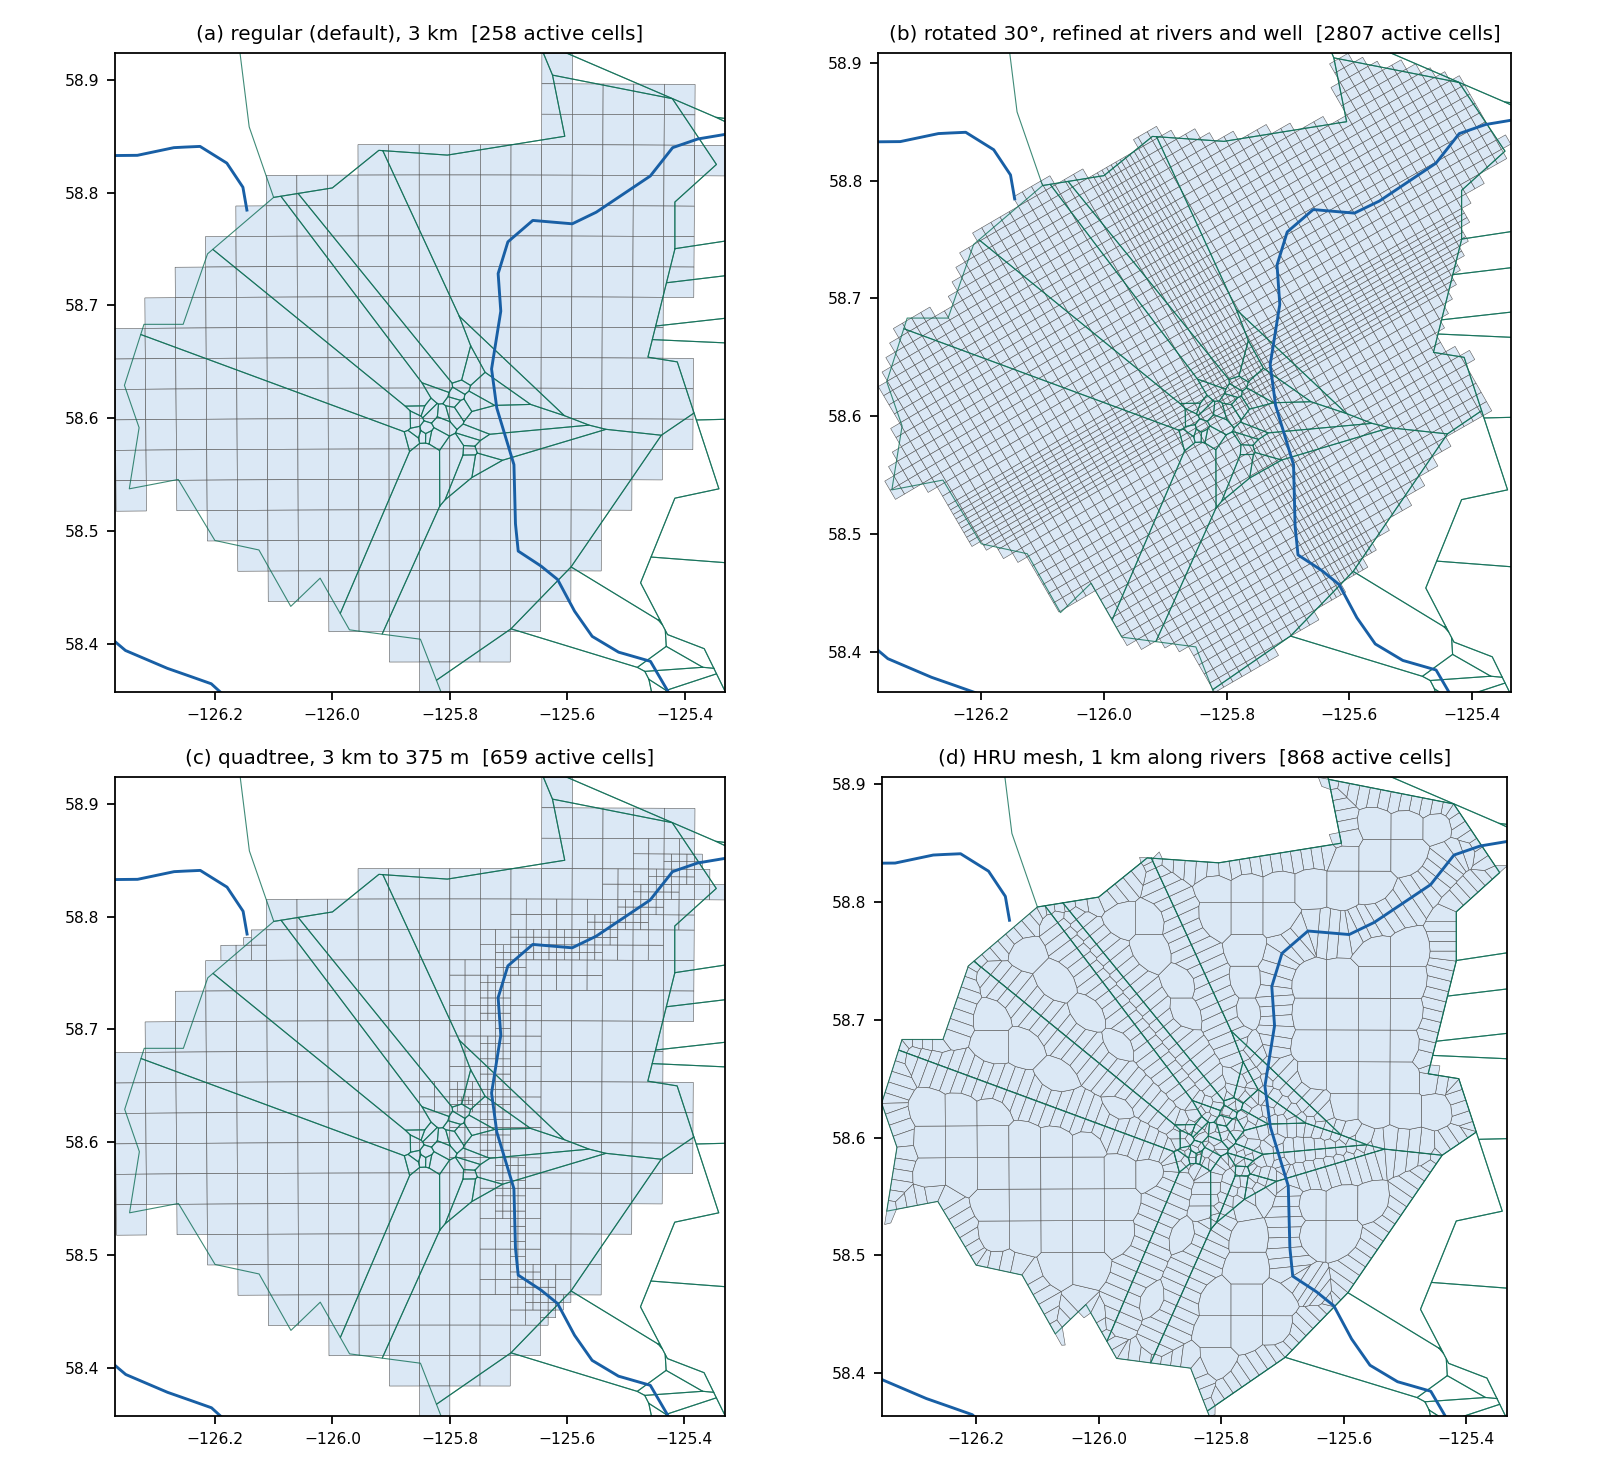
\includegraphics[width=0.78\linewidth]{figures/fig_grids.png}
\caption{The same model (Liard subbasin 52, HRU boundaries green, rivers blue) on four grids: (a) the default regular
grid; (b) rotated 30\textdegree{} and refined along rivers and around a well; (c) a quadtree refined along rivers and around the
well; (d) an HRU mesh whose cells follow HRU boundaries, with cells along the rivers.}\label{fig:ugrids}
\end{figure}
Figure~\ref{fig:ugrids} shows four of them.
\begin{table}[!htbp]\centering
\caption{Grid options and what to write in the \cmd{.rvg} file.}\label{tab:ugridtypes}
\begin{tabularx}{\linewidth}{P{0.25\linewidth}P{0.33\linewidth}Y}\toprule\hdr
Option & What to write & Use it when\\\midrule
Regular (default) & nothing, or \cmd{:GridType REGULAR} & a first model; uniform cells are enough\\
Rotated, refined & \cmd{:GridRotation 20}, \cmd{:GridRefinement RIVERS 1000} & a valley has a clear direction; finer rows and columns near rivers or wells\\
Quadtree & \cmd{:GridType QUADTREE} with \cmd{:GridRefinement} & fine cells only where they matter, few cells elsewhere\\
HRU mesh & \cmd{:GridType HRU\_MESH} & cells should follow HRU boundaries\\
Imported cells & \cmd{:GridType FILE}, \cmd{:GridFile cells.geojson} & a grid made elsewhere (FloPy, gridgen, ModelMuse, QGIS)\\
Layers by elevation & \cmd{:LayerConnection ELEVATION} & layers of neighbouring profiles should connect where they lie at the same elevation\\\bottomrule
\end{tabularx}
\end{table}
Start with the default grid and a cell size of a few kilometres. Refine where heads and exchanges change quickly: along
rivers that gain or lose much water, around pumping wells, around lakes and reservoirs, and in wetlands. Reference,
Section~\ref{R-sec:gridtypes}, describes each option. Every run writes \cmd{mf6/grid\_cells.geojson}, each cell as a
polygon ready to be joined with heads in QGIS.

\subsection{Choosing a grid for the Liard model}\label{sec:liardgrids}
The Liard model was run for two years on each grid option (Table~\ref{tab:liardgrids}). Every run keeps the water accounts
exact (MODFLOW residual about $10^{-11}$, no failed step, Raven's balance unchanged).
\begin{table}[!htbp]\centering
\caption{The Liard model (2 years) on each grid: active cells, run time on one core, Nash--Sutcliffe efficiency at 10BE004 /
10BE005 / 10BE010, mean seepage to Raven and mean net aquifer discharge to rivers [million m$^3$/d].}\label{tab:liardgrids}
\begin{tabular}{lrrcrr}\toprule\hdr
Grid & Cells & Time [s] & NSE & Seepage & Rivers\\\midrule
Regular 2 km (default) & 8\,840 & 40 & 0.728 / 0.861 / 0.635 & 9.48 & 0.82\\
Regular, rotated 20\textdegree, 1 km along rivers & 35\,058 & 220 & 0.726 / 0.861 / 0.638 & 9.92 & 0.66\\
Quadtree 2 km, 500 m along rivers & 16\,276 & 108 & 0.719 / 0.858 / 0.611 & 9.49 & 0.01\\
HRU mesh 2 km, 1 km along rivers & 14\,610 & 100 & 0.717 / 0.859 / 0.627 & 9.94 & 0.35\\
Regular 2 km, layers by elevation & 8\,840 & 41 & 0.666 / 0.859 / 0.606 & 4.11 & 0.49\\
\bottomrule\end{tabular}
\par\smallskip\footnotesize MODFLOW 6.8.1 (\cmd{tests/liard\_grids.py}); run times on one core of the test machine.
\end{table}
Streamflow hardly changes: total seepage is nearly the same on every grid, and the river exchange is a small part of the
flow at the gauges.

The net river exchange, however, depends on the size of the river cells: 0.82 million m$^3$/d with 2 km cells, 0.01 with
500 m cells. There are two reasons. The channel bed is placed at the lowest DEM value along the river in each cell,
which is lower in larger cells. And the head of a large cell averages the aquifer over a wider area around the river.
So calibrate the riverbed parameters (\cmd{RIVERBED\_K}, \cmd{:RiverBedDepth}) on the grid that will be used, and
compare models only at the same river-cell size.

Connecting layers by elevation halves the seepage here, because water in the upland till can flow directly into the
valley gravel where the two lie at the same elevation. That is a different conceptual model rather than a refinement. A
regular grid refined to 1 km along rivers has more than twice the cells of a quadtree with 500 m river cells, because its
refinement spans whole rows and columns.

\section{Starting heads}\label{sec:ustart}
Raven needs a head in every cell on the first day. It takes, in this order:
\begin{enumerate}
\item the heads of a hotstart file (\cmd{:GWHeads} in the \cmd{.rvc} file, Chapter~\ref{uch:restarts});
\item \cmd{:InitialGWHeads DEPTH\_BELOW\_SURFACE d} or \cmd{:InitialGWHeads ELEVATION z} in the \cmd{.rvc} file;
\item each profile's \cmd{INITIAL\_HEAD\_DEPTH} below the land surface.
\end{enumerate}
Guessed heads can be far from reality. \cmd{:GWInitialization STEADY\_STATE r} in the \cmd{.rvg} file first solves a
steady state with a recharge of $r$~mm/d over the area of the coupled HRUs, before Raven's first day. If that steady state
does not converge (for example when wells pump more than the aquifer can supply), Raven warns and starts from the initial
heads instead. Reference, Section~\ref{R-sec:init}, gives the details.

\section{Wells, monitoring wells and boundaries}\label{sec:uwells}
\begin{whattowrite}
\small In the \cmd{.rvg} file:
\begin{lstlisting}
:Wells
  :Attributes, NAME, LATITUDE, LONGITUDE, SCREEN_TOP, SCREEN_BOT
  1, PW_1, 59.27310, -124.73460, 1199.7, 1188.7
:EndWells
:ObservationWells
  :Attributes, NAME, LATITUDE, LONGITUDE, SCREEN_ELEV
  101, OW_NEAR, 59.27310, -124.73060, 1192.7
:EndObservationWells
:GeneralHeadBoundary   GHB1  boundary_line.geojson HEAD 1310.0 CONDUCTANCE 5000.0 LAYERS TOP
:SpecifiedHeadBoundary LAKE1 lake.geojson          HEAD 1312.0 LAYERS TOP
\end{lstlisting}
and in the \cmd{.rvt} file \cmd{:WellFlowRate 1 m3/d} (negative = pumping), \cmd{:BoundaryHead GHB1 m} (replaces
\cmd{HEAD}) and \cmd{:ObservationData GW\_HEAD 101 m}.
\end{whattowrite}
\begin{itemize}
\item \textbf{Wells} pump from (or inject into) the layers their screen crosses; the rate is split among the layers by
their transmissivity. A well rate series must cover the whole simulation, like every Raven forcing series. MODFLOW lowers
the rate of a well whose cell runs dry, and \cmd{GWBudget.csv} reports the specified and the actual rates.
\item \textbf{Monitoring wells} report the simulated head at their screen (\cmd{GWHeads.csv}) and are scored against
\cmd{:ObservationData GW\_HEAD} in \cmd{Diagnostics.csv}, like streamflow.
\item \textbf{Head-dependent boundaries} (\cmd{:GeneralHeadBoundary}) exchange water with a water body outside the model,
in proportion to the head difference. \textbf{Fixed-head boundaries} (\cmd{:SpecifiedHeadBoundary}) hold the head of their
cells.
\item A boundary is drawn in a GeoJSON file: polygons select the cells whose centre lies inside, lines the cells they
cross. \cmd{LAYERS ALL} (the default) places it in every active layer whose bottom lies below its head, \cmd{LAYERS TOP}
in the highest such layer. So the \cmd{HEAD} (or the \cmd{:BoundaryHead} series) must lie above the bottoms of the cells
it is to hold.
\item Two \cmd{:SpecifiedHeadBoundary} commands that select the same cell stop the run, naming both. General-head
boundaries may share cells.
\end{itemize}
Reference, Section~\ref{R-ch:wells}, gives the rules.

\section{Setting up your own model}\label{ch:ownmodel}
\subsection{A groundwater file to start from}
\begin{whattowrite}
\small
\begin{lstlisting}
# my.rvg - the groundwater file of a model Raven builds
:HRUGeometry        my_hrus.geojson   HRU_ID     # required
:RiverGeometry      my_rivers.geojson SubId      # river lines, subbasin ID field optional
:LandSurface        dem.tif                      # DEM
:BedrockSurface     bedrock.tif                  # or DEFAULT_BEDROCK_DEPTH of the profiles
:GridCellSize       1000.0                       # m
:GWInitialization   STEADY_STATE 0.5             # steady start, mean recharge [mm/d]
:HeadSaveFrequency  30
\end{lstlisting}
\end{whattowrite}
Add wells, monitoring wells, boundaries, wetlands and reservoirs as you need them. Reference, Section~\ref{R-ch:c6}, ends
with a groundwater file that uses most options.

\subsection{Checklist}
\begin{enumerate}
\item \textbf{HRU polygons.} Export the HRU polygons from your GIS or BasinMaker as GeoJSON in longitude/latitude
(EPSG:4326), or in their projection with \cmd{:InputCRS}, with a field holding the HRU ID used in the \cmd{.rvh} file.
\item \textbf{Maps.} A DEM and a bedrock (or aquifer-base) elevation map as GeoTIFF files or ESRI ASCII grids in
longitude/latitude (or in the projection of \cmd{:InputCRS}), in the same vertical datum. River lines as GeoJSON.
\item \textbf{Profiles.} Group your HRUs by the aquifer beneath them and write one profile per group; set
\cmd{AQUIFER\_PROFILE} in the \cmd{.rvh}.
\item \textbf{Recharge.} Decide which Raven flux is recharge (usually percolation from the deepest soil store) and send it
to \cmd{GROUNDWATER} for coupled HRUs only. Remove or restrict any process that drains \cmd{GROUNDWATER} there, and any
conceptual baseflow that would double-count groundwater.
\item \textbf{Grid size.} Choose $\Delta$ so that the smallest features you care about span a few cells, but the number of
active cells stays manageable (a few thousand to a few hundred thousand per layer).
\item \textbf{Start.} Use \cmd{:GWInitialization STEADY\_STATE} with the long-term average recharge, or a warm-up period.
\item \textbf{Check.} Read \cmd{GWModelSummary.txt} and run \cmd{tools\_audit.py} (Section~\ref{sec:uaudit}).
\item \textbf{Calibrate.} Use streamflow and monitoring-well heads (Section~\ref{ch:calib}).
\end{enumerate}

\subsection{Typical parameter values}
Typical values for aquifer materials are listed in Reference, Section~\ref{R-app:materials}, and typical ranges for every
aquifer class and profile parameter in Reference, Sections~\ref{R-app:class} and~\ref{R-app:profile}.

\subsection{How much of the water balance should groundwater take?}
In a coupled HRU, Raven's conceptual baseflow from deep stores is replaced by MODFLOW. Check after a first run that the
long-term baseflow (seepage plus aquifer discharge to rivers) is plausible, and that the aquifer is not steadily filling or
emptying (storage release near zero on average once spin-up is over).
